% !TeX spellcheck = pl_PL-Polish
\documentclass[12pt,a4paper]{article}

\usepackage[T1]{fontenc}
\usepackage[polish]{babel}
\usepackage[utf8]{inputenc}
\usepackage{lmodern}
\selectlanguage{polish}
\usepackage{graphicx}
\usepackage{xcolor}
\usepackage{float}
\usepackage{url}

\def\projectName{Wdrażanie i zarządzanie aplikacjami w klastrze AKS}
\def\authorA{Wiktor Jarosz}
\def\authorB{Andrzej Machnik}
\def\authorC{Tomasz Solarz}
\newcommand\todo[1]{\textcolor{red}{#1}}

\begin{document}
\pagenumbering{gobble}
\clearpage
	\begin{figure}[h]
		\centering
		%
\includegraphics[width=0.5\linewidth]{media/polsl_logo_pion_en_rgb.png}
		
\includegraphics[width=0.5\linewidth]{media/ps-logo.png}
	\end{figure}

\hspace{3cm}
	\begin{center}Dokumentacja projektowa\end{center}
	\hspace{3cm}
	\begin{center}\large\textbf{Zarządzanie Systemami Informatycznymi}\end{center}
	\begin{center}\large\textit{\projectName}\end{center}

\hspace{7cm}
	\begin{flushright}Kierunek: Informatyka
		\end{flushright}
		\begin{flushright}Członkowie zespołu:
		\par
		\textit{\authorA}
		\par
		\textit{\authorB}
		\par
		\textit{\authorC}
	\end{flushright}
\vfill
	\begin{center}Gliwice, 2025/2026\end{center}

\newpage
\pagenumbering{arabic}
\tableofcontents





\newpage
\section{Wprowadzenie}
\subsection{Role w projekcie}
	W ramach projektu wyznaczono trzy główne role, odpowiadające poszczególnym etapom cyklu życia aplikacji w chmurze:
	\begin{itemize}
		\item \textbf{Wiktor Jarosz (Osoba 1)} -- Inżynier Infrastruktury. Odpowiada za przygotowanie i konfigurację środowiska chmurowego Azure Kubernetes Service (AKS), zarządzanie grupami zasobów oraz uprawnieniami dostępu (RBAC).
		\item \textbf{Andrzej Machnik (Osoba 2)} -- Inżynier DevOps. Odpowiada za deployment aplikacji (serwer nginx), automatyzację procesów wdrażania, przeprowadzenie aktualizacji typu \textit{rolling update} oraz finalną redakcję dokumentacji technicznej.
		\item \textbf{Tomasz Solarz (Osoba 3)} -- Inżynier QA i Niezawodności. Odpowiada za testowanie dostępności aplikacji (np. skryptami \texttt{curl}), analizę logów systemowych, ocenę niezawodności rozwiązania oraz przeprowadzenie i weryfikację scenariusza awaryjnego (\textit{rollback}).
	\end{itemize}

\subsection{Cel projektu}
	Celem projektu jest demonstracja procesu ciągłego wdrażania aplikacji w środowisku Kubernetes (AKS) z zachowaniem wysokiej dostępności. Kluczowe aspekty obejmują:
	\begin{itemize}
		\item Uruchomienie klastra AKS jako fundamentu pod aplikacje kontenerowe.
		\item Wdrożenie przykładowego serwera WWW (nginx) i wystawienie go na świat.
		\item Przeprowadzenie bezawaryjnej aktualizacji aplikacji (\textit{rolling update}).
		\item Symulację awarii (wadliwa aktualizacja) oraz szybki powrót do stabilnej wersji (\textit{rollback}).
	\end{itemize}

\subsection{Streszczenie}
	Projekt skupia się na praktycznym wykorzystaniu narzędzi \texttt{az cli} oraz \texttt{kubectl} do zarządzania infrastrukturą chmurową. Pokazuje, jak mechanizmy natywne dla Kubernetesa wspierają niezawodność i pozwalają na bezpieczne zarządzanie wersjami oprogramowania.





\newpage
\section{Założenia projektowe}
\subsection{Założenia techniczne i nietechniczne}
	\ldots 

\subsection{Stos technologiczny}
	W projekcie wykorzystano następujące narzędzia i technologie:
	\begin{itemize}
		\item \textbf{Microsoft Azure} -- platforma chmurowa udostępniająca usługę AKS.
		\item \textbf{Azure Kubernetes Service (AKS)} -- zarządzane środowisko Kubernetes.
		\item \textbf{Azure CLI (\texttt{az})} -- interfejs wiersza poleceń do zarządzania zasobami Azure.
		\item \textbf{kubectl} -- narzędzie do zarządzania klastrami Kubernetes.
		\item \textbf{Nginx} -- serwer WWW wykorzystany jako aplikacja testowa.
		\item \textbf{Bash/cURL} -- narzędzia do testowania dostępności i skryptowania testów.
	\end{itemize}

\subsection{Oczekiwane rezultaty projektu}
	Głównym rezultatem jest stabilnie działająca aplikacja na klastrze AKS, która potrafi przetrwać proces aktualizacji bez przestojów. Dodatkowo, zespół wypracuje procedurę wycofywania zmian w przypadku wykrycia błędów w nowej wersji oprogramowania.





\newpage
\section{Realizacja projektu}
	Opis wszystkich etapów realizacji projektu obejmuje przygotowanie infrastruktury, wdrożenie aplikacji oraz testy niezawodności.

	\subsection{Przygotowanie środowiska}
	Pierwszym krokiem projektu jest przygotowanie środowiska --- zarówno tego chmurowego, jak i lokalnego. Środowisko lokalne to aplikacja Azure CLI, którą należy pobrać zgodnie z instrukcją na stronie Microsoft. Dla systemów Linux, instrukcja ta znajduje się pod URL https://learn.microsoft.com/en-us/cli/azure/install-azure-cli-linux.

	\begin{figure}[h!]
		\centering
		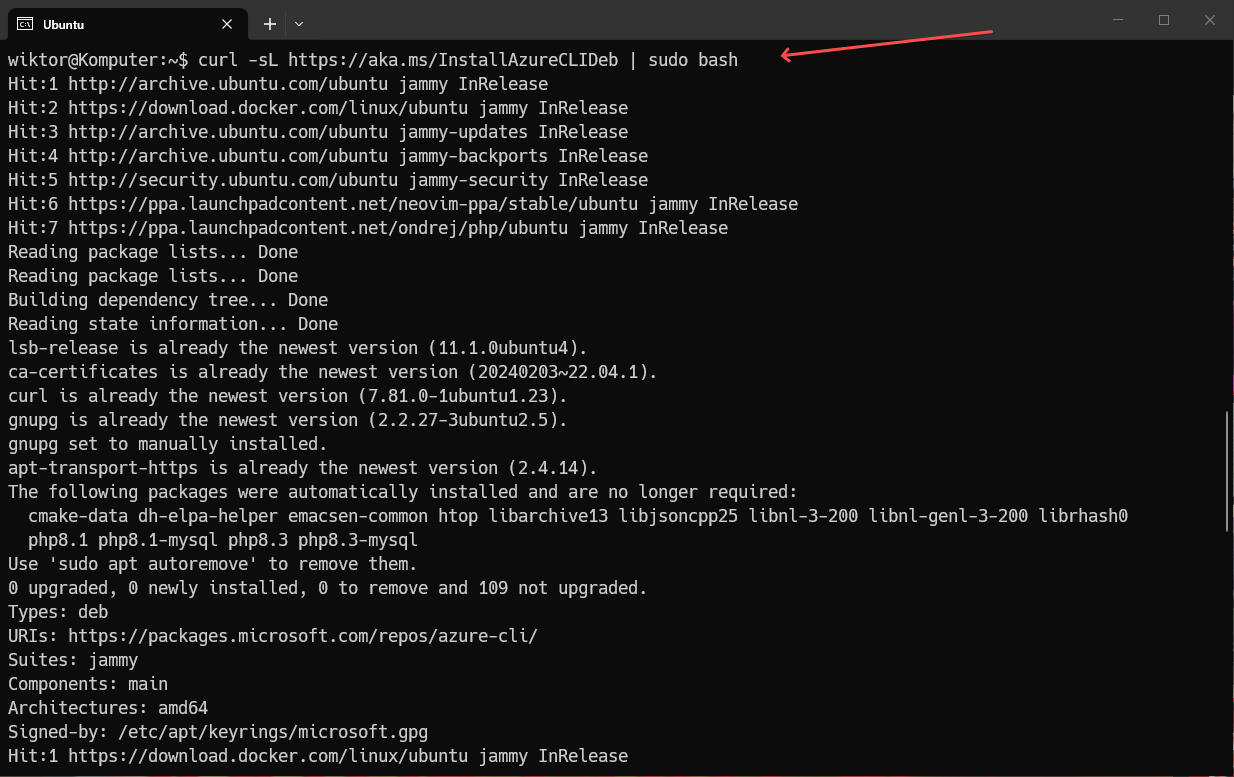
\includegraphics[width=1.0\linewidth]{media/instalacja-azure-cli.png}
		\caption{Przykładowa instalacja Azure CLI w systemie Ubuntu}
		\label{fig:instalacja_cli}
	\end{figure}

	Aby zalogować się z poziomu terminala do konta Microsoft, należy użyć polecenia \texttt{az login}, które sprawi, że otwarta zostanie strona logowania w przeglądarce (flaga \texttt{use-device-code} musi zostać użyta, gdy na systemie nie ma zainstalowanej przeglądarki).

	\begin{figure}[h!]
		\centering
		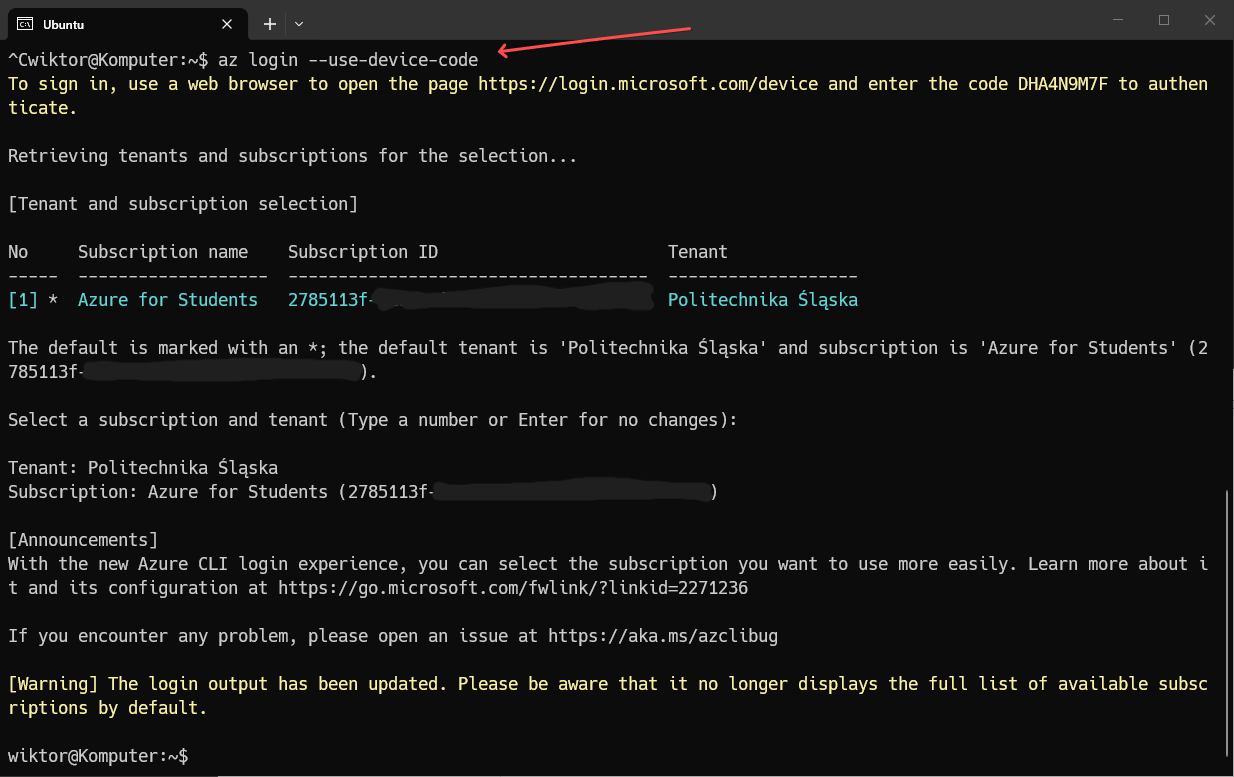
\includegraphics[width=1.0\linewidth]{media/logowanie-cli.png}
		\caption{Logowanie do konta Azure}
		\label{fig:logowanie_cli}
	\end{figure}

	W środowisku lokalnym zainstalowane musi być również narzędzie kubectl służące do zarządzania klastrem AKS. Instalacja odbywa się komendą \texttt{sudo az aks install-cli}.

	\begin{figure}[h!]
		\centering
		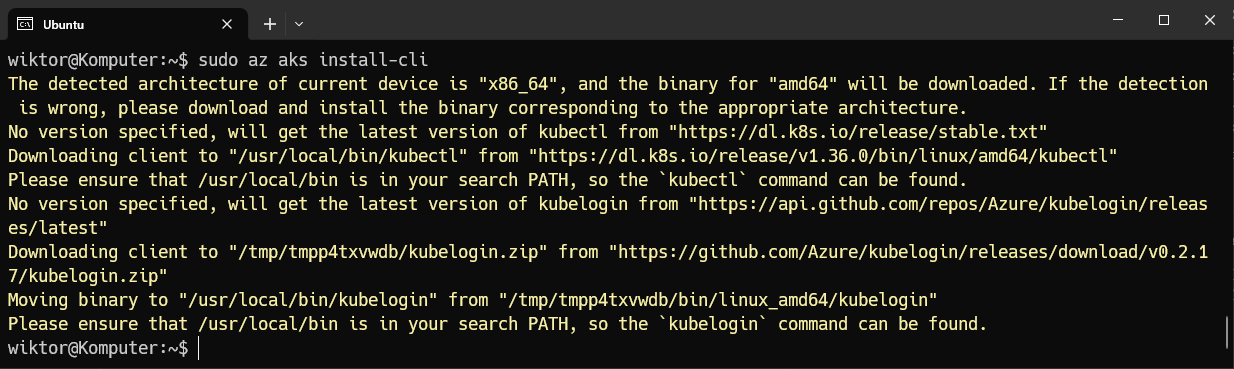
\includegraphics[width=1.0\linewidth]{media/instalacja-kubectl.png}
		\caption{Instalacja kubectl}
		\label{fig:instalacja_kubectl}
	\end{figure}

	Po udanej konfiguracji środowiska lokalnego oraz zalogowaniu do konta Azure, następnym krokiem jest utworzenie grupy zasobów (ang. resource group). Grupy zasobów to logiczne foldery grupujące powiązane usługi chmurowe. Pozwalają one na ich organizację oraz na łatwiejsze zarządzanie (podobnie jak katalogi w systemach operacyjnych).

	\begin{figure}[h!]
		\centering
		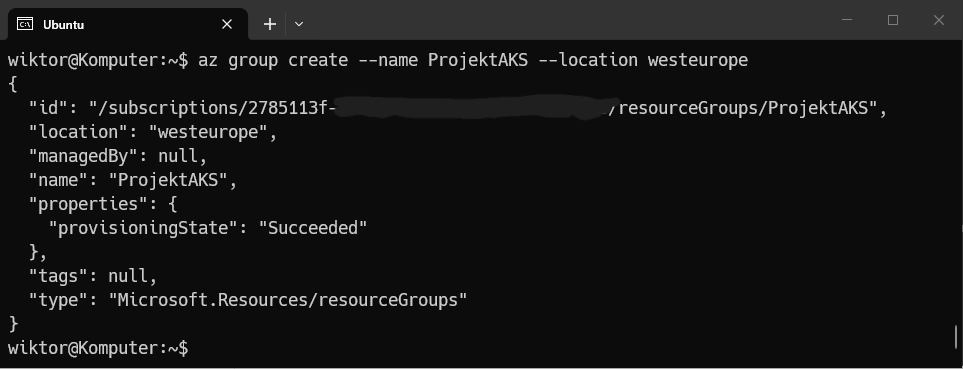
\includegraphics[width=1.0\linewidth]{media/resource-group.png}
		\caption{Utworzenie grupy zasobów "ProjektAKS" na serwerach \textit{westeurope}}
		\label{fig:resource_group}
	\end{figure}

	W celu utworzenia klastra, wymagane jest aktywowanie na koncie Azure modułu pozwalającego na zarządzanie usługami kontenerowymi (o ile moduł ten nie jest jeszcze aktywny). Aby to zrobić, należy wykonać polecenie \verb|az provider register --namespace Microsoft.ContainerService|. Rejestracja usługi trwa zazwyczaj kilka minut, po czym możliwe jest utworzenie klastra. Na ilustracji \ref{fig:klaster} widać proces tworzenia klastra zawierającego 2 węzły w rozmiarze \texttt{Standard\_B2s}, które mają 2 vCPU, 4 GB RAM oraz 8 GB przestrzeni dyskowej.

	\begin{figure}[h!]
		\centering
		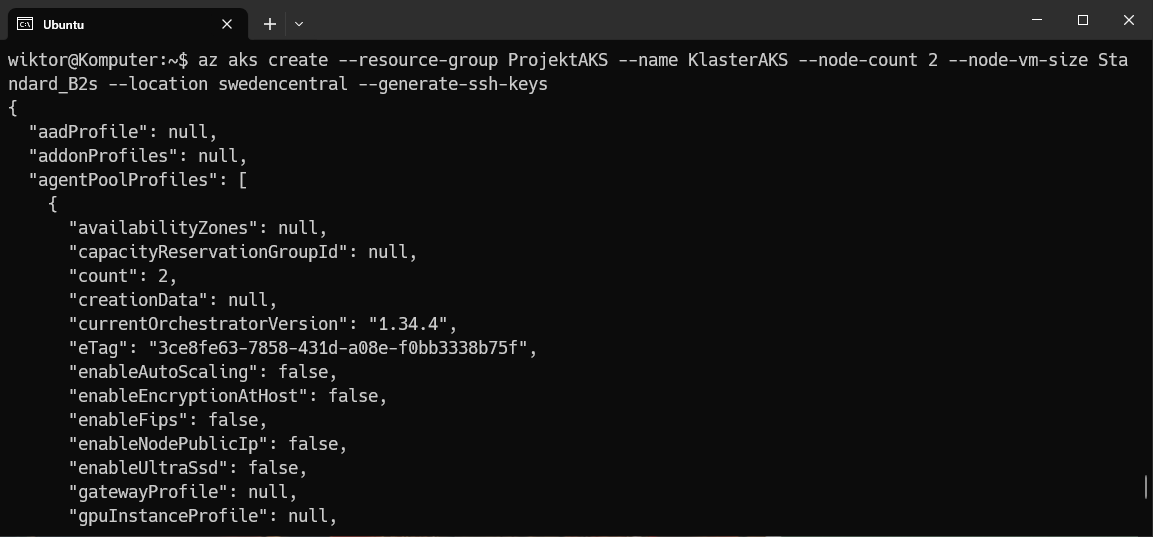
\includegraphics[width=1.0\linewidth]{media/utworzenie-klastra.png}
		\caption{Utworzenie klastra "KlasterAKS" z dwoma węzłami Standard\_B2s}
		\label{fig:klaster}
	\end{figure}

	\begin{figure}[h!]
		\centering
		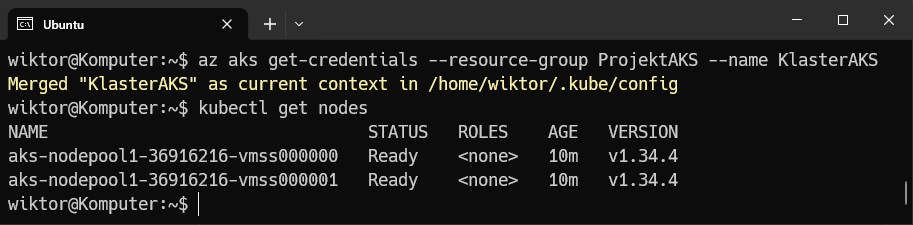
\includegraphics[width=1.0\linewidth]{media/weryfikacja-wezlow.png}
		\caption{Pobranie danych logowania oraz weryfikacja działania węzłów}
		\label{fig:weryfikacja-wezlow}
	\end{figure}

	Ostatnim krokiem w przygotowaniu środowiska jest nadanie dostępu do klastra członkom zespołu zgodnie z zasadą najmniejszego uprzywilejowania (ang. principle of least privilege). Najprościej zrobić to z poziomu panelu web Azure, co widać na ilustracji \ref{fig:dostep}.

	\begin{figure}[h!]
		\centering
		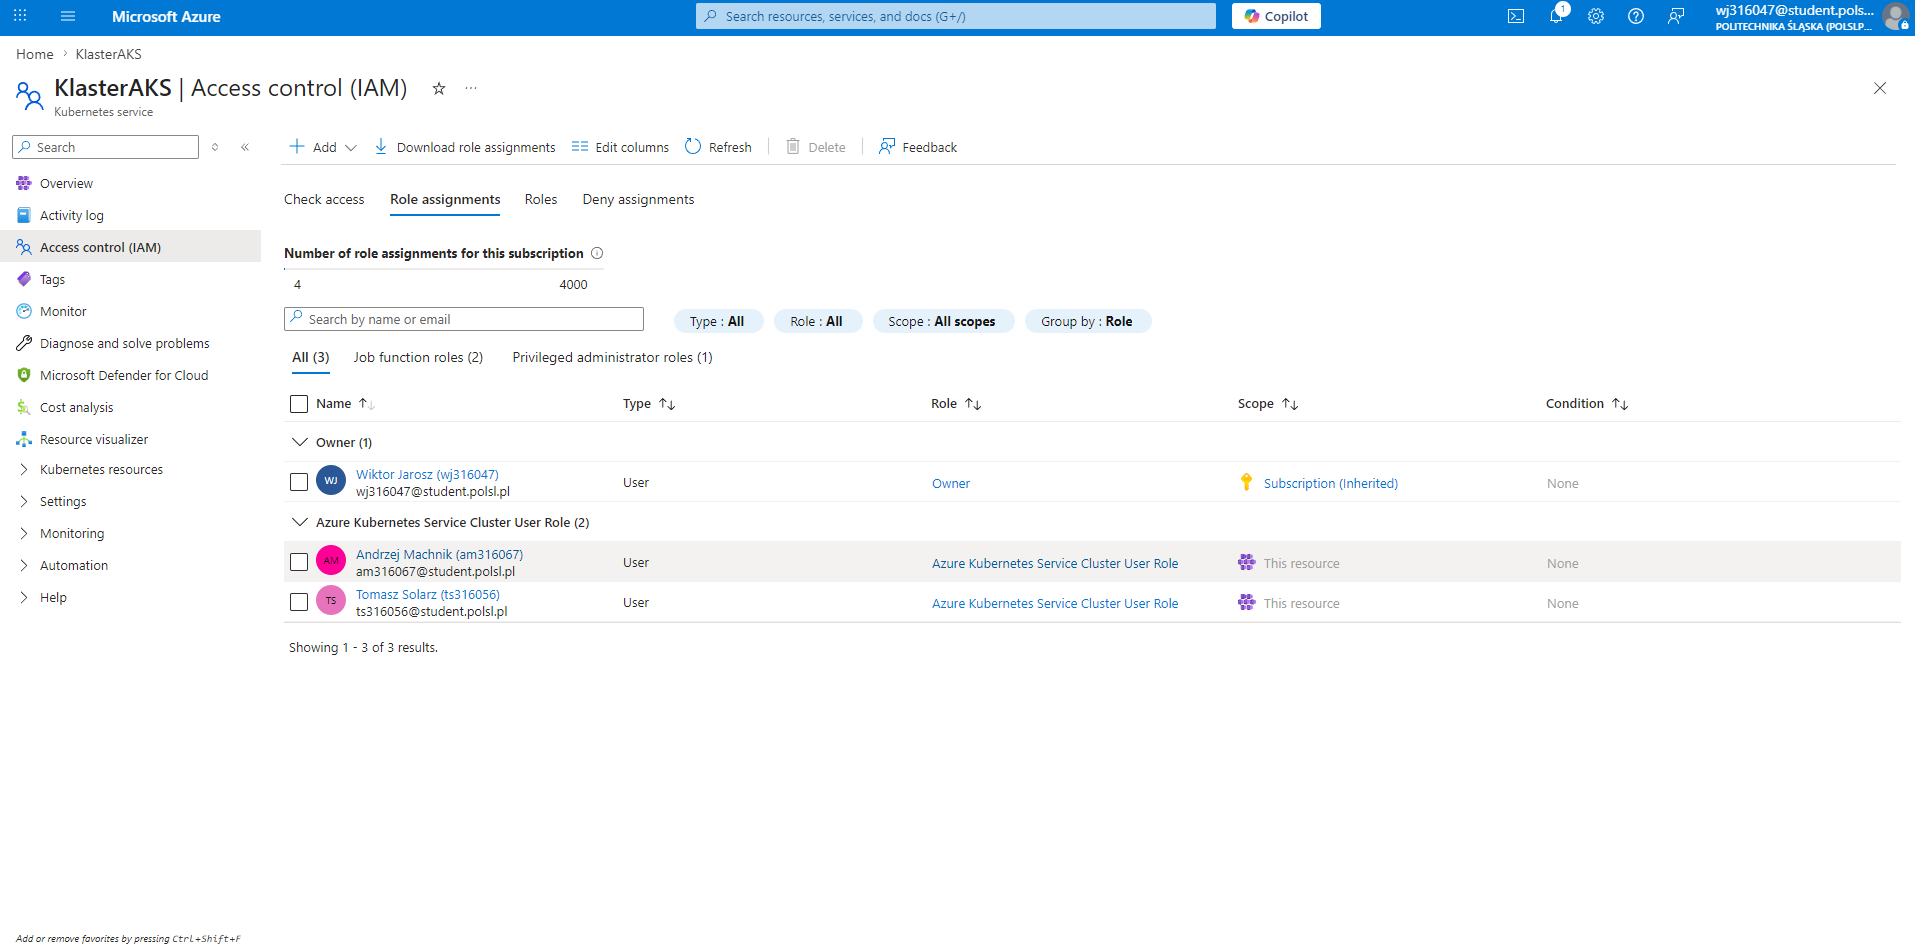
\includegraphics[width=1.0\linewidth]{media/dostep.png}
		\caption{Nadanie dostępu do klastra członkom zespołu}
		\label{fig:dostep}
	\end{figure}

	\subsection{Wdrożenie aplikacji i Rolling Update}
	Andrzej Machnik (Osoba 2) przeprowadził proces wdrożenia aplikacji webowej opartej na obrazie \texttt{nginx:1.20}. Proces ten obejmował:
	\begin{itemize}
		\item Utworzenie manifestu \texttt{deployment.yaml} z określoną liczbą replik (3) oraz strategią \textit{RollingUpdate}.
		\item Skonfigurowanie serwisu typu \texttt{LoadBalancer}, aby wystawić aplikację na publicznym adresie IP.
		\item Przeprowadzenie aktualizacji do wersji \texttt{nginx:1.21} poprzez komendę \texttt{kubectl set image}.
	\end{itemize}
	Dzięki zastosowaniu parametrów \texttt{maxSurge} oraz \texttt{maxUnavailable}, klaster Kubernetes był w stanie wymieniać kontenery pojedynczo, zachowując ciągłość obsługi zapytań użytkowników.

	\subsection{Testy dostępności i analiza logów}
	Tomasz Solarz (Osoba 3) weryfikował poprawność procesu aktualizacji oraz stabilność środowiska po zmianach.
	
	\begin{figure}[h!]
		\centering
		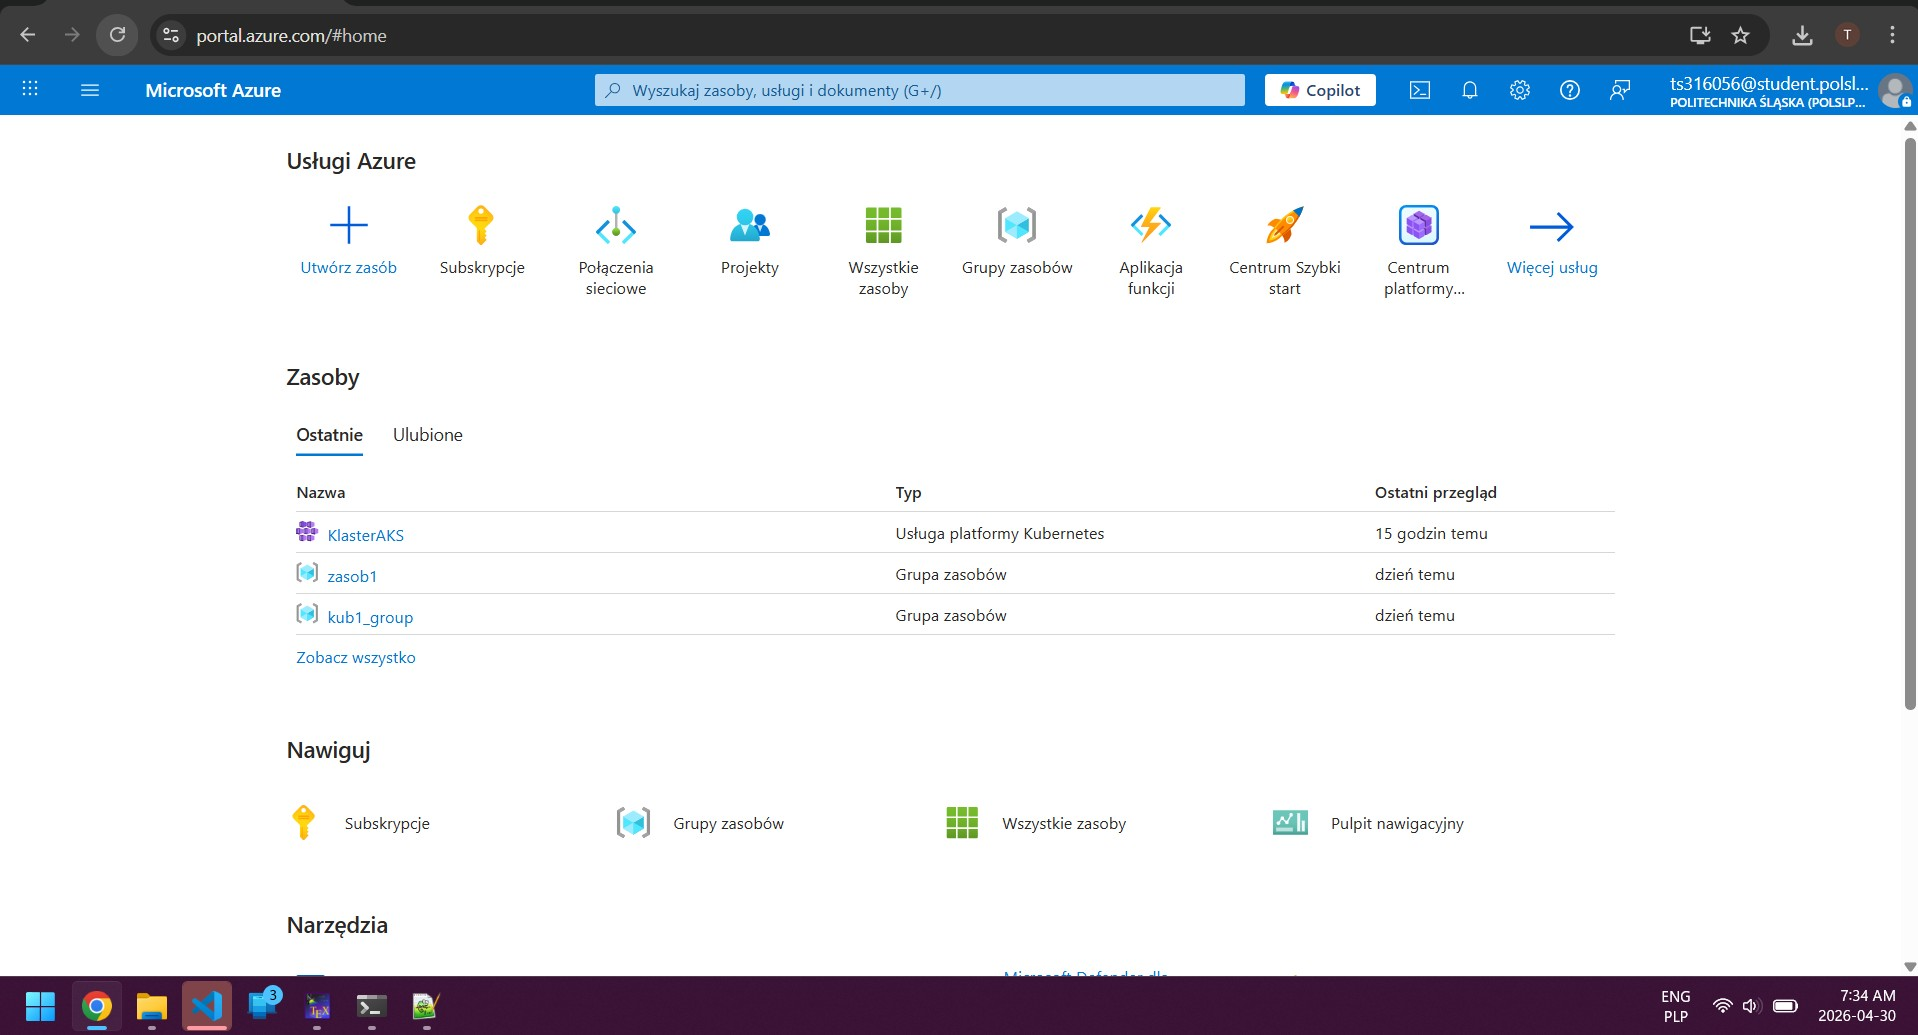
\includegraphics[width=1.0\linewidth]{media/s1.jpg}
		\caption{Azure web GUI}
		\label{fig:start}
	\end{figure}

	\subsubsection{Testowanie dostępności skryptami cURL}
	W celu potwierdzenia braku przestojów, uruchomiono skrypt monitorujący kod odpowiedzi HTTP:
	\begin{verbatim}
	while true; do 
	  STATUS=$(curl -s -o /dev/null -w "%{http_code}" http://<EXTERNAL_IP>)
	  echo "Status: $STATUS - $(date)"
	  if [ "$STATUS" -ne 200 ]; then echo "BŁĄD!"; fi
	  sleep 0.5
	done
	\end{verbatim}
	Podczas całego procesu \textit{rolling update}, skrypt nie zarejestrował ani jednego zapytania zakończonego błędem, co dowodzi poprawnej konfiguracji strategii wdrażania.

	\subsubsection{Analiza logów i ocena niezawodności}
	Po wdrożeniu nowej wersji, przeanalizowano logi za pomocą \texttt{kubectl logs -l app=nginx}. Skupiono się na:
	\begin{itemize}
		\item Weryfikacji komunikatów startowych serwera nginx (brak błędów konfiguracji).
		\item Monitorowaniu logów dostępu pod kątem równomiernego rozłożenia ruchu pomiędzy nowe pody.
		\item Sprawdzeniu logów zdarzeń klastra (\texttt{kubectl get events}), co potwierdziło płynne usuwanie starych i tworzenie nowych instancji kontenerów.
	\end{itemize}
	Na tej podstawie oceniono niezawodność rozwiązania jako wysoką, spełniającą standardy systemów krytycznych.

	\subsection{Scenariusz awaryjny i Rollback}
	Aby przetestować odporność systemu na błędy ludzkie lub błędy w kodzie, Tomasz Solarz przeprowadził symulację awarii.

	\subsubsection{Wdrożenie wadliwej wersji}
	Do klastra próbowano wdrożyć wersję aplikacji z błędnym tagiem obrazu (\texttt{nginx:non-existent-tag}). Kubernetes, zgodnie z polityką \textit{RollingUpdate}, uruchomił nowy pod, jednak po wykryciu błędu \texttt{ImagePullBackOff}, wstrzymał dalszą wymianę instancji, chroniąc system przed całkowitym paraliżem.

	\subsubsection{Przeprowadzenie procedury Rollback}
	W celu natychmiastowego przywrócenia pełnej sprawności, wykonano wycofanie zmian:
	\begin{verbatim}
	kubectl rollout undo deployment/nginx-deployment
	\end{verbatim}
	
	\begin{figure}[h!]
		\centering
		\includegraphics[width=1.0\linewidth]{media/s3.png}
		\caption{Udana procedura}
		\label{fig:rollback}
	\end{figure}
	
	Po wykonaniu tej komendy, klaster automatycznie powrócił do ostatniej stabilnej konfiguracji. Cała operacja trwała kilka sekund i nie wpłynęła na dostępność usługi dla użytkowników końcowych.


\newpage
\section{Wnioski}
	Realizacja projektu pozwoliła na wyciągnięcie następujących wniosków:
	\begin{itemize}
		\item \textbf{Wysoka dostępność:} Mechanizm \textit{rolling update} w Kubernetesie pozwala na aktualizację oprogramowania bez przerywania świadczenia usług, co jest kluczowe w nowoczesnych systemach IT.
		\item \textbf{Szybkość odzyskiwania:} Funkcja \textit{rollback} umożliwia niemal natychmiastowy powrót do działającej wersji aplikacji w przypadku awarii nowej wersji, co minimalizuje czas przestoju.
		\item \textbf{Zalety AKS:} Wykorzystanie zarządzanego klastra AKS znacznie upraszcza administrację infrastrukturą, pozwalając zespołowi skupić się na wdrażaniu i utrzymaniu aplikacji.
		\item \textbf{Monitorowanie:} Analiza logów jest niezbędnym elementem procesu wdrażania, pozwalającym na wczesne wykrycie anomalii po aktualizacji.
	\end{itemize}





\newpage
\section{Bibliografia}
\begin{enumerate}
	\item Microsoft Learn, \textit{Dokumentacja usługi Azure Kubernetes Service (AKS)}, [online] \url{https://learn.microsoft.com/pl-pl/azure/aks/} (dostęp: 30.04.2026).
	\item Kubernetes Documentation, \textit{Deployments - Strategy: Rolling Update}, [online] \url{https://kubernetes.io/docs/concepts/workloads/controllers/deployment/#rolling-update-deployment} (dostęp: 30.04.2026).
	\item Kubernetes Documentation, \textit{Rolling Back a Deployment}, [online] \url{https://kubernetes.io/docs/concepts/workloads/controllers/deployment/#rolling-back-a-deployment} (dostęp: 30.04.2026).
	\item Nginx Inc., \textit{Nginx Open Source User Guide}, [online] \url{https://docs.nginx.com/nginx/admin-guide/} (dostęp: 30.04.2026).
	\item B. Beyer, C. Jones, J. Petoff, N. R. Murphy, \textit{Site Reliability Engineering: How Google Runs Production Systems}, O'Reilly Media, 2016.
	\item Microsoft Learn, \textit{Zasada najmniejszego uprzywilejowania (Principle of Least Privilege)}, [online] \url{https://learn.microsoft.com/pl-pl/windows-server/identity/ad-ds/plan/security-best-practices/implementing-least-privilege-administrative-models} (dostęp: 30.04.2026).
\end{enumerate}

\end{document}